\documentclass[12pt,a4paper]{article}
\usepackage[utf8]{inputenc}
\usepackage[T1]{fontenc}
\usepackage[brazil]{babel}
\usepackage{geometry}
\usepackage{graphicx}
\usepackage{float}
\usepackage{booktabs}
\usepackage{hyperref}
\usepackage{helvet}
\renewcommand{\familydefault}{\sfdefault}

\geometry{margin=2.5cm}
\graphicspath{{./figuras/}}
\setcounter{secnumdepth}{0}

\title{Relatorio - Exercicio 1\\Visualizacao de dados da OMS com abordagem de redes}
\author{Aluno(a): \rule{7cm}{0.4pt}}
\date{\today}

\begin{document}

\maketitle

\section{Objetivo}
Neste relatorio, a ideia foi pegar os dados de Covid-19 da OMS e transformar em redes para facilitar a leitura. Em vez de olhar so para tabela, usamos grafos para enxergar melhor como paises e regioes se relacionam em termos de casos e obitos.

\section{Base de dados utilizada}
\textbf{Fonte:} OMS - dashboard Covid-19\\
\textbf{Arquivo:} \texttt{WHO-COVID-19-global-table-data.csv}\\
\textbf{Unidade de analise:} paises e regioes OMS

As variaveis principais usadas no script foram:
\begin{itemize}
  \item casos acumulados e casos por 100 mil habitantes;
  \item casos recentes (7 dias e 24 horas, quando disponiveis);
  \item obitos acumulados e obitos por 100 mil habitantes;
  \item obitos recentes (7 dias e 24 horas, quando disponiveis).
\end{itemize}

\section{Etapas realizadas}
\subsection{1) Importacao e organizacao dos dados}
Primeiro, o arquivo CSV foi lido no R e organizado em um \texttt{data.frame}. Depois disso:
\begin{itemize}
  \item houve padronizacao dos nomes das colunas;
  \item variaveis numericas foram convertidas para formato numerico;
  \item regioes vazias foram marcadas como \texttt{Unknown};
  \item registros agregados (ex.: \texttt{Global} e \texttt{International conveyance}) foram removidos para evitar vieses.
\end{itemize}

\subsection{2) Preparacao para visualizacao em rede}
Para os grafos ficarem mais claros e uteis na analise:
\begin{itemize}
  \item foram aplicados filtros de completude de dados (\texttt{NA});
  \item foram usados recortes dos paises com maior relevancia epidemiologica em algumas estrategias;
  \item foram calculadas medidas de similaridade/proximidade por distancia euclidiana em dados padronizados;
  \item foi calculado o indicador \textit{CFR} (\textit{case fatality ratio}) em uma das redes.
\end{itemize}

\subsection{3) Geracao de imagens}
As visualizacoes foram exportadas em alta resolucao (300 DPI) para a pasta \texttt{figuras}, com legendas e rotulos de nos em cor preta para melhorar a leitura.

\section{Visualizacoes produzidas e interpretacao}

\subsection{Estrategia A - Rede bipartida Regiao-Pais}
\begin{figure}[H]
\centering
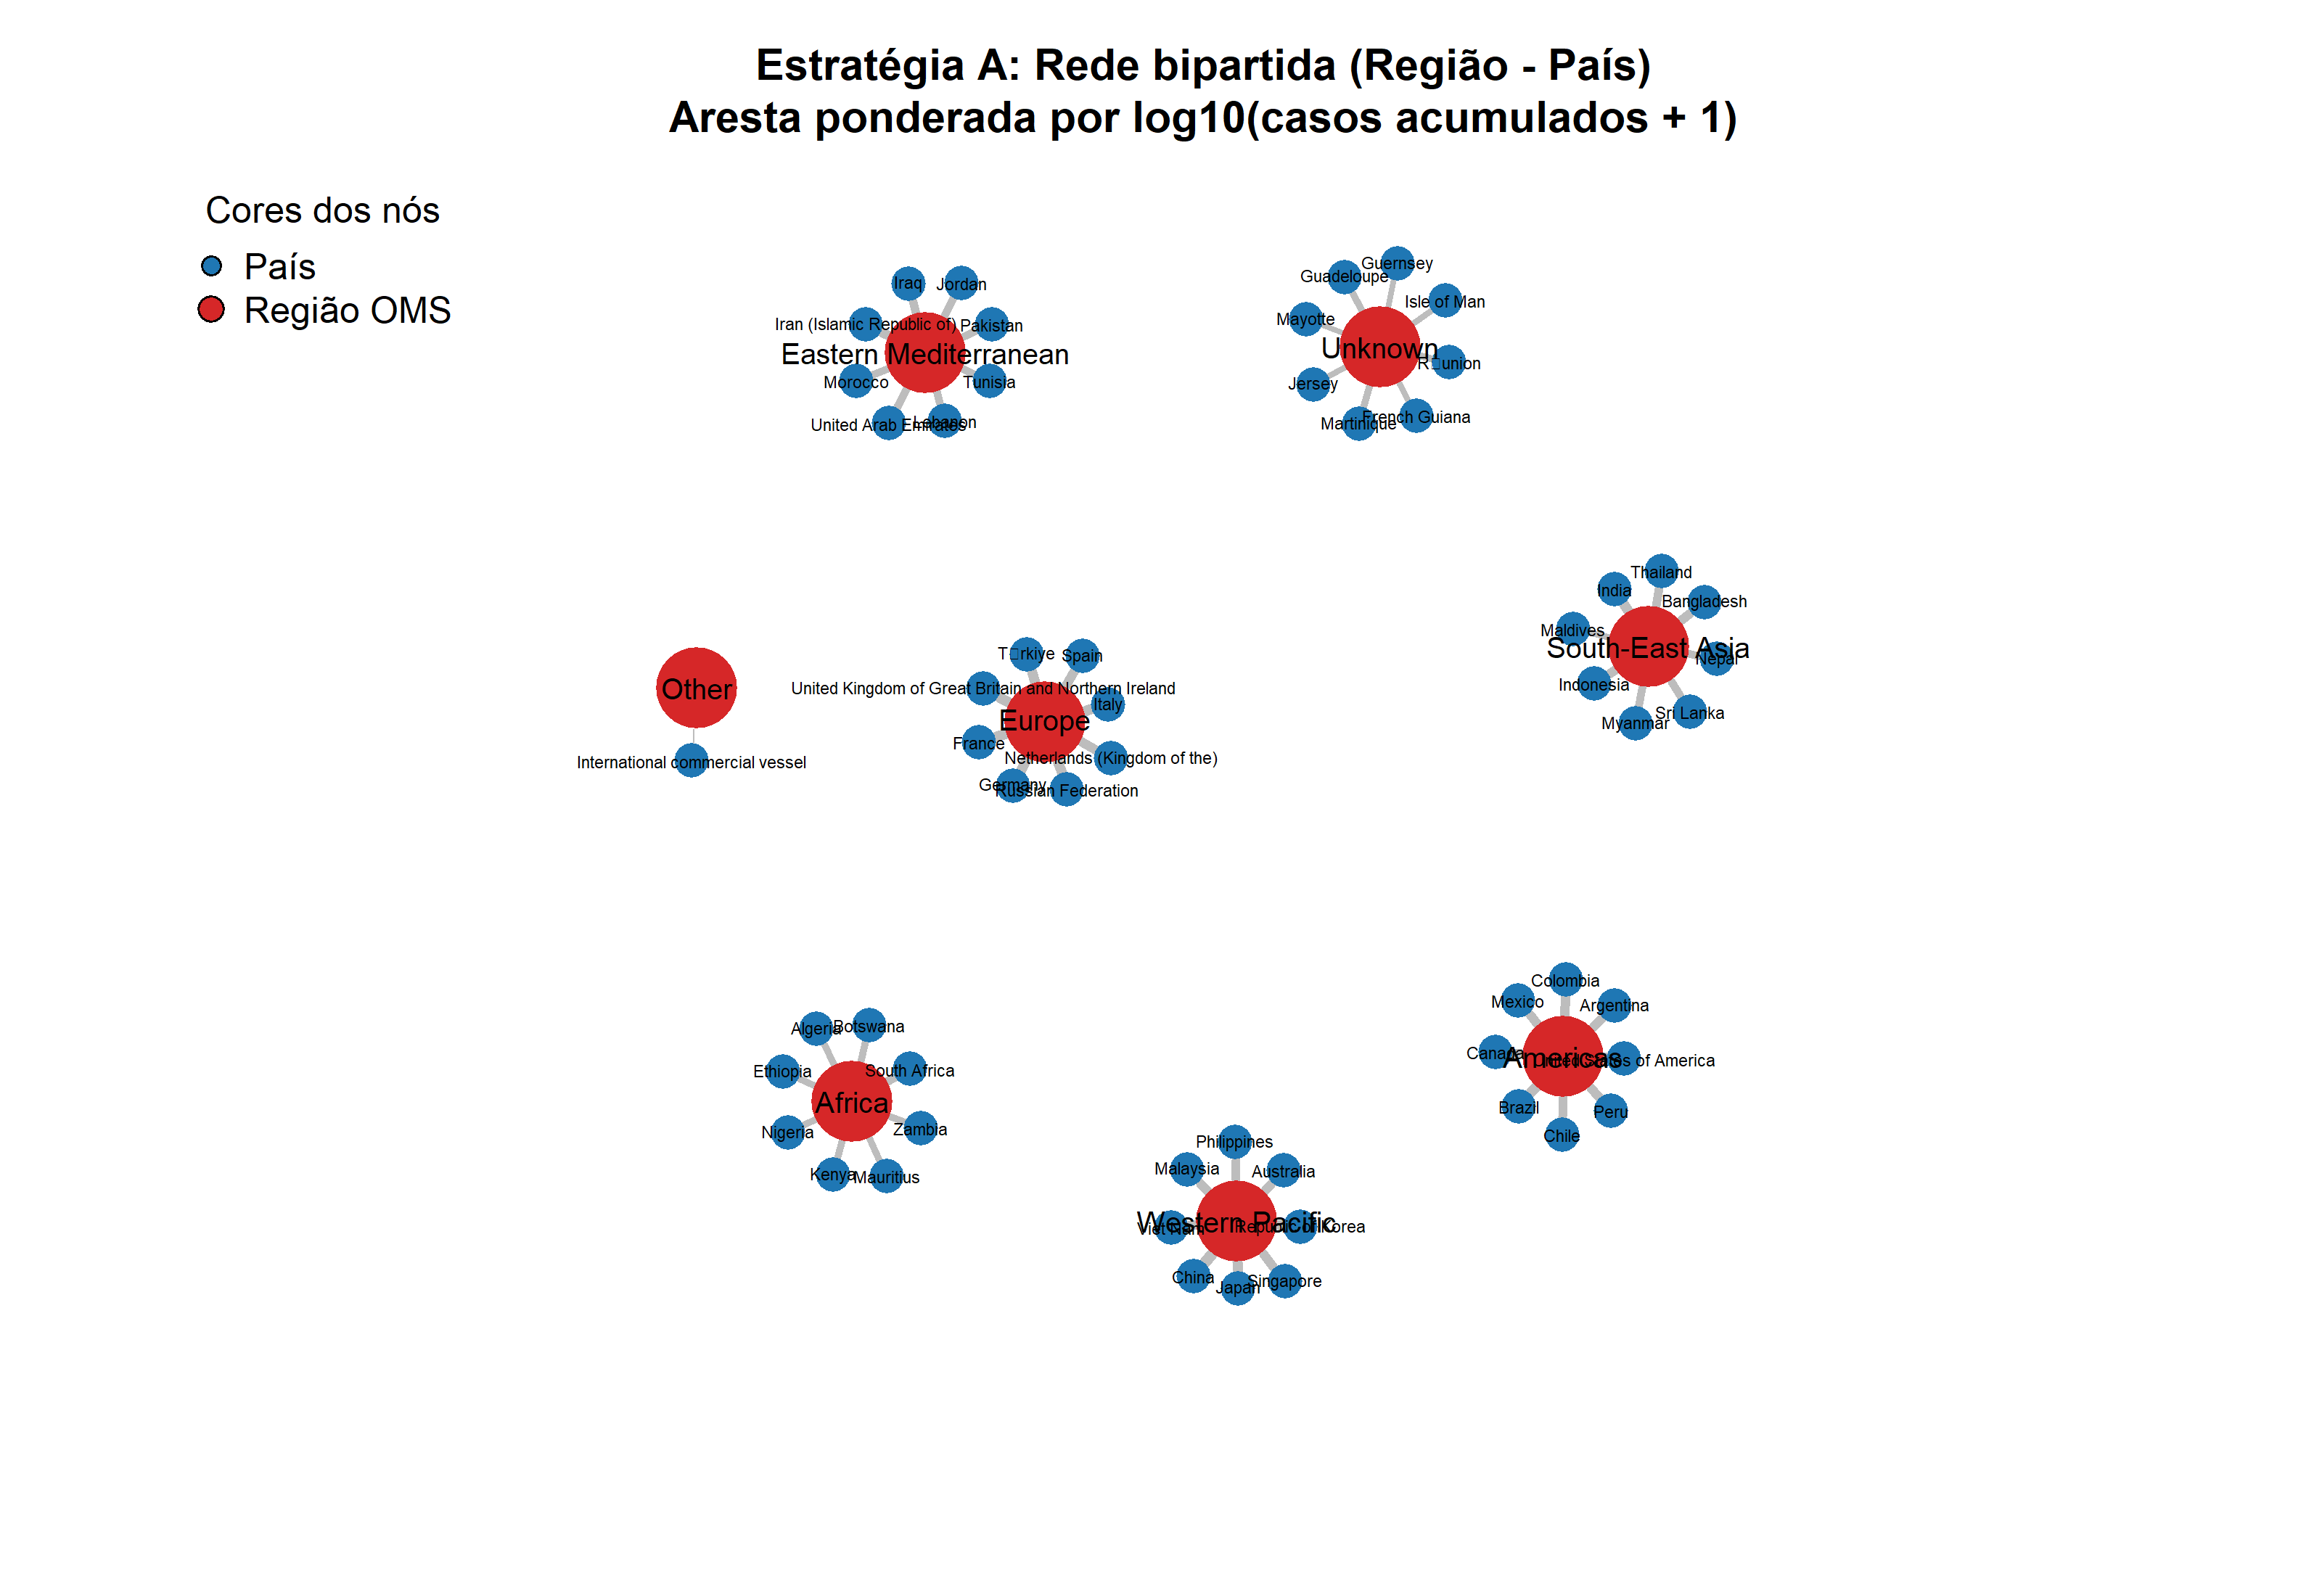
\includegraphics[width=0.98\textwidth]{rede_bipartida_regiao_pais.png}
\caption{Rede bipartida entre Regioes OMS e paises, com arestas ponderadas por carga de casos acumulados.}
\end{figure}

\textbf{Interpretacao (linguagem simples):}
\begin{itemize}
  \item Essa rede mostra quem esta ligado a quem: regiao de um lado e pais do outro.
  \item Quanto mais forte a conexao, maior o peso de casos acumulados naquele pais.
  \item Da para ver rapido onde a carga ficou mais concentrada dentro de cada regiao.
\end{itemize}

\subsection{Estrategia B - Rede de similaridade entre regioes}
\begin{figure}[H]
\centering
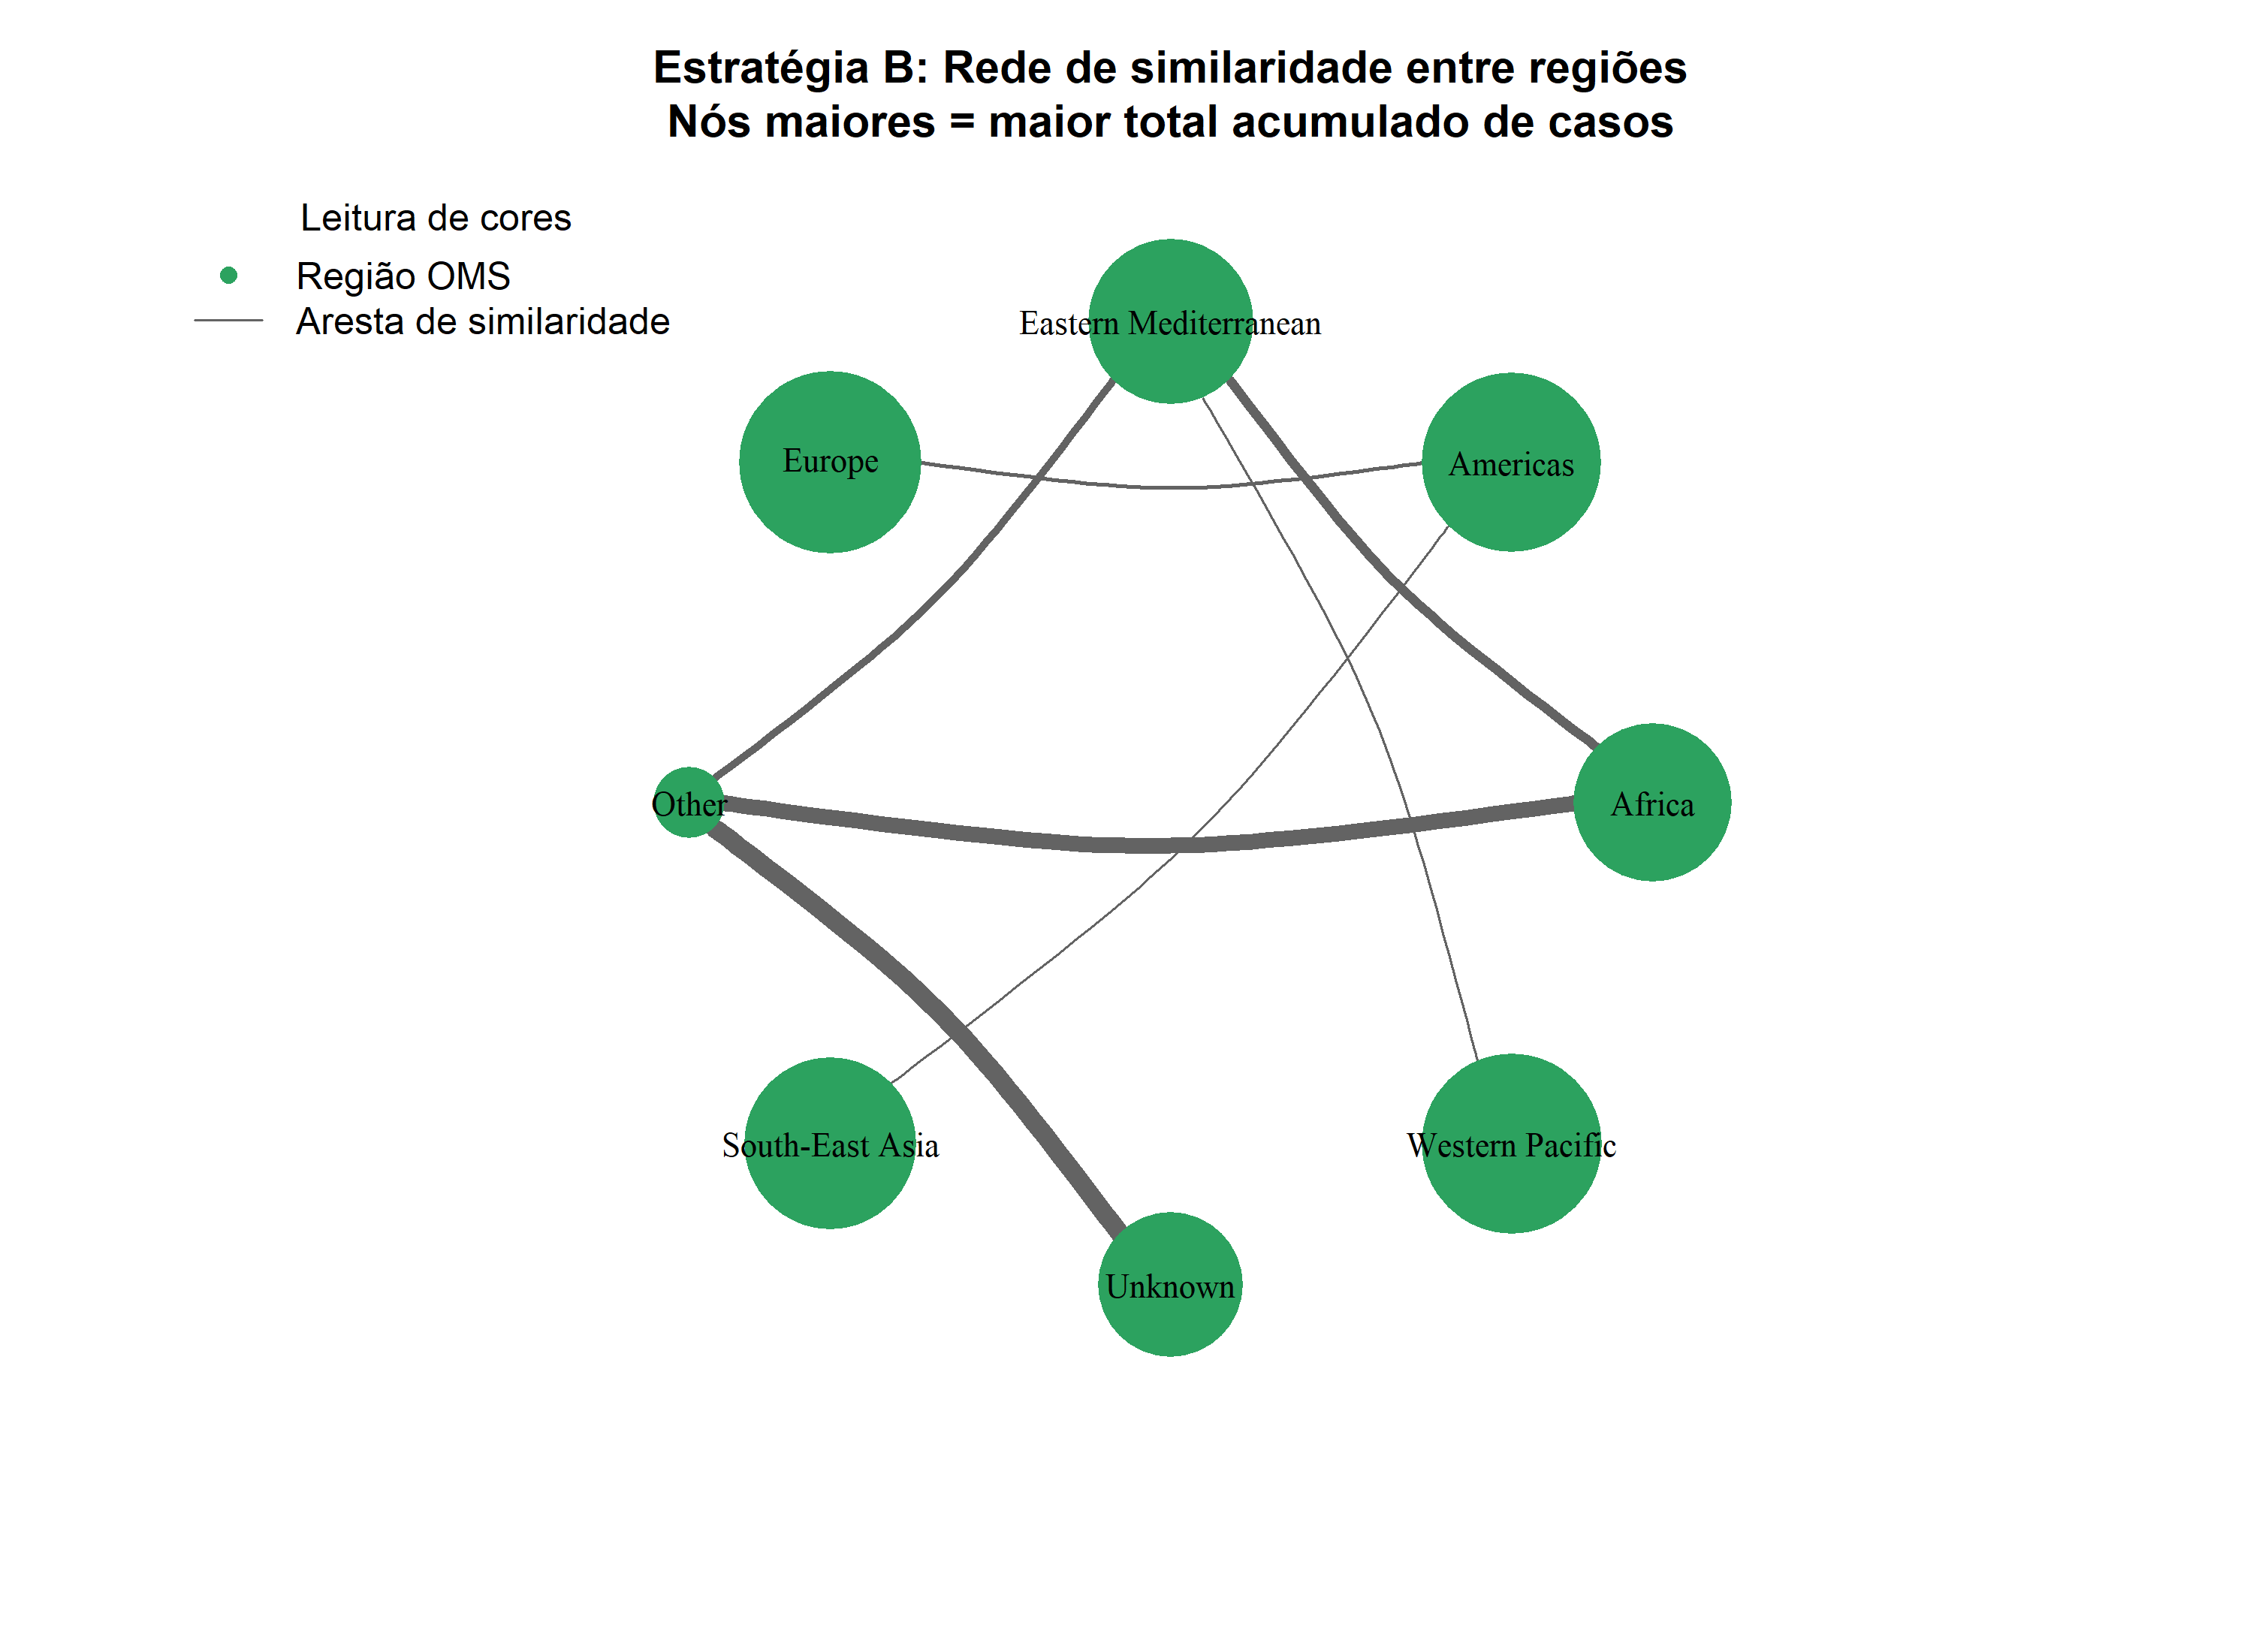
\includegraphics[width=0.90\textwidth]{rede_similaridade_regioes.png}
\caption{Rede de similaridade entre regioes OMS baseada em indicadores medios de casos e obitos.}
\end{figure}

\textbf{Interpretacao (linguagem simples):}
\begin{itemize}
  \item Aqui cada no e uma regiao da OMS.
  \item Regioes mais conectadas entre si tem comportamento parecido nos indicadores medios.
  \item E uma forma direta de comparar regioes sem precisar olhar varios numeros separados.
\end{itemize}

\subsection{Estrategia C - Rede de proximidade entre paises (k-NN)}
\begin{figure}[H]
\centering
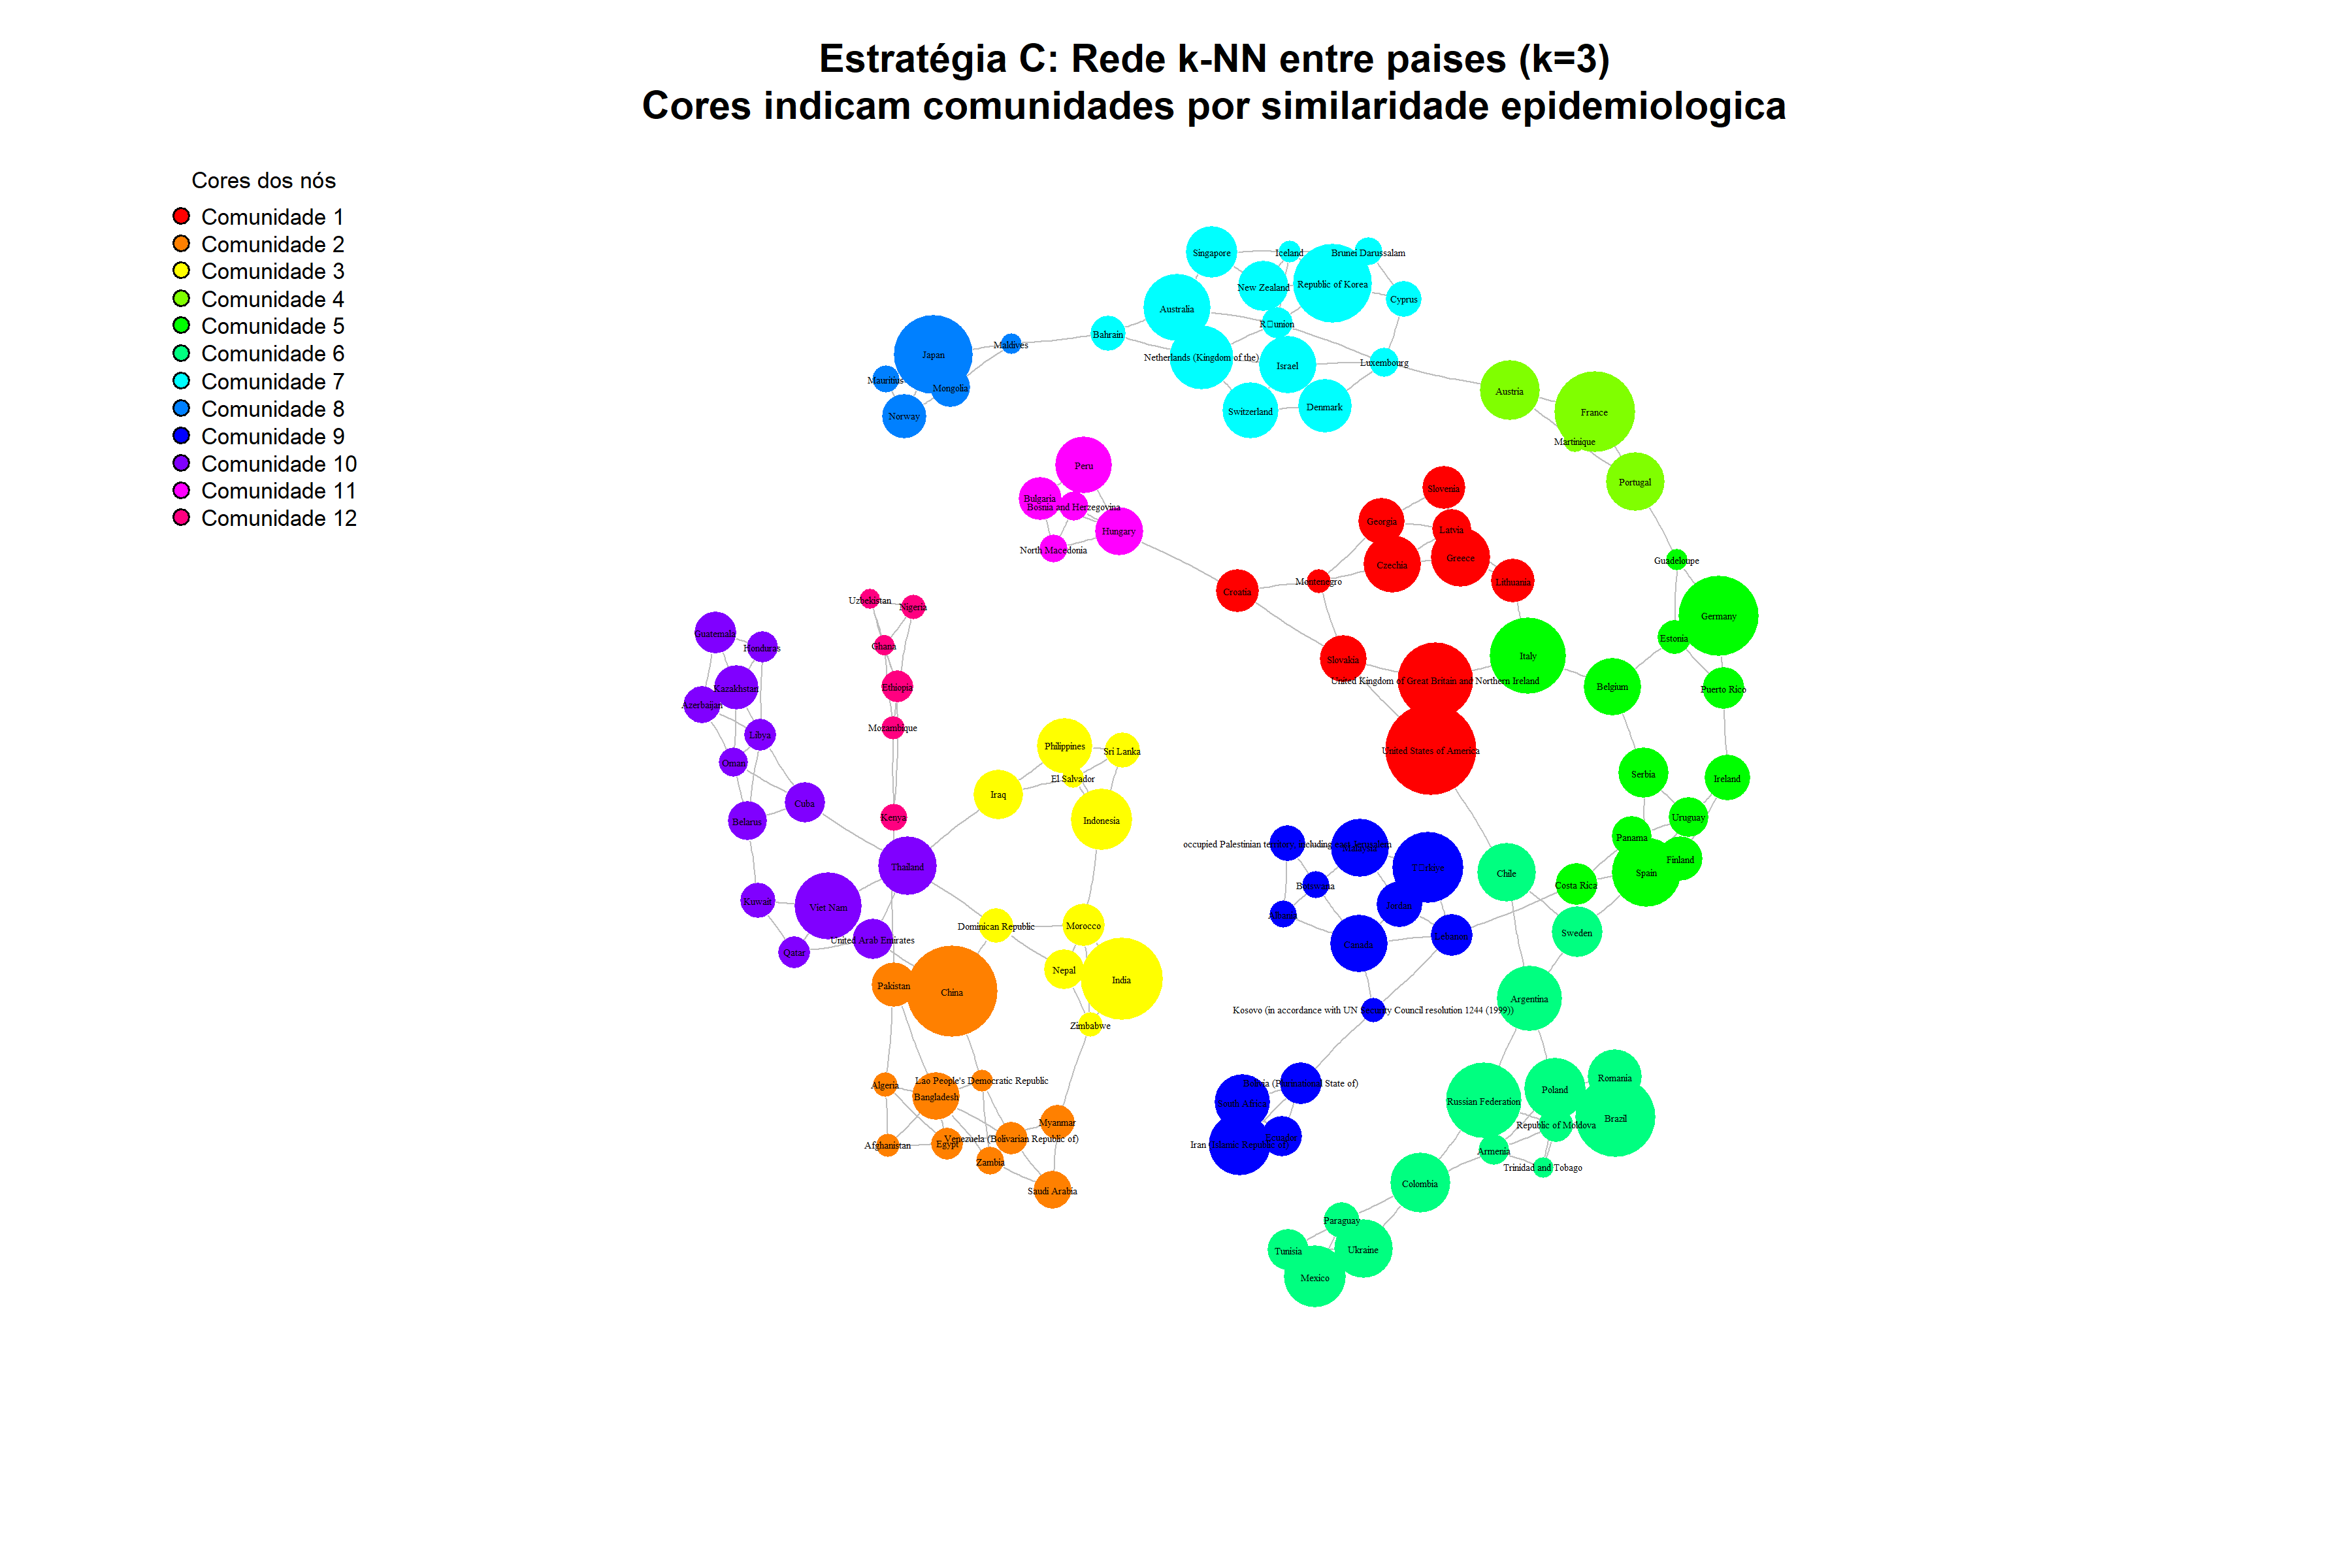
\includegraphics[width=0.98\textwidth]{rede_proximidade_paises_knn.png}
\caption{Rede k-NN entre paises; as cores representam comunidades detectadas por similaridade.}
\end{figure}

\textbf{Interpretacao (linguagem simples):}
\begin{itemize}
  \item Cada pais foi ligado aos vizinhos mais parecidos (k-NN).
  \item As cores mostram grupos (comunidades) com padrao per capita parecido.
  \item Mesmo paises longe no mapa podem cair no mesmo grupo se os numeros forem parecidos.
\end{itemize}

\subsection{Estrategia D - Rede de perfil de carga e letalidade}
\begin{figure}[H]
\centering
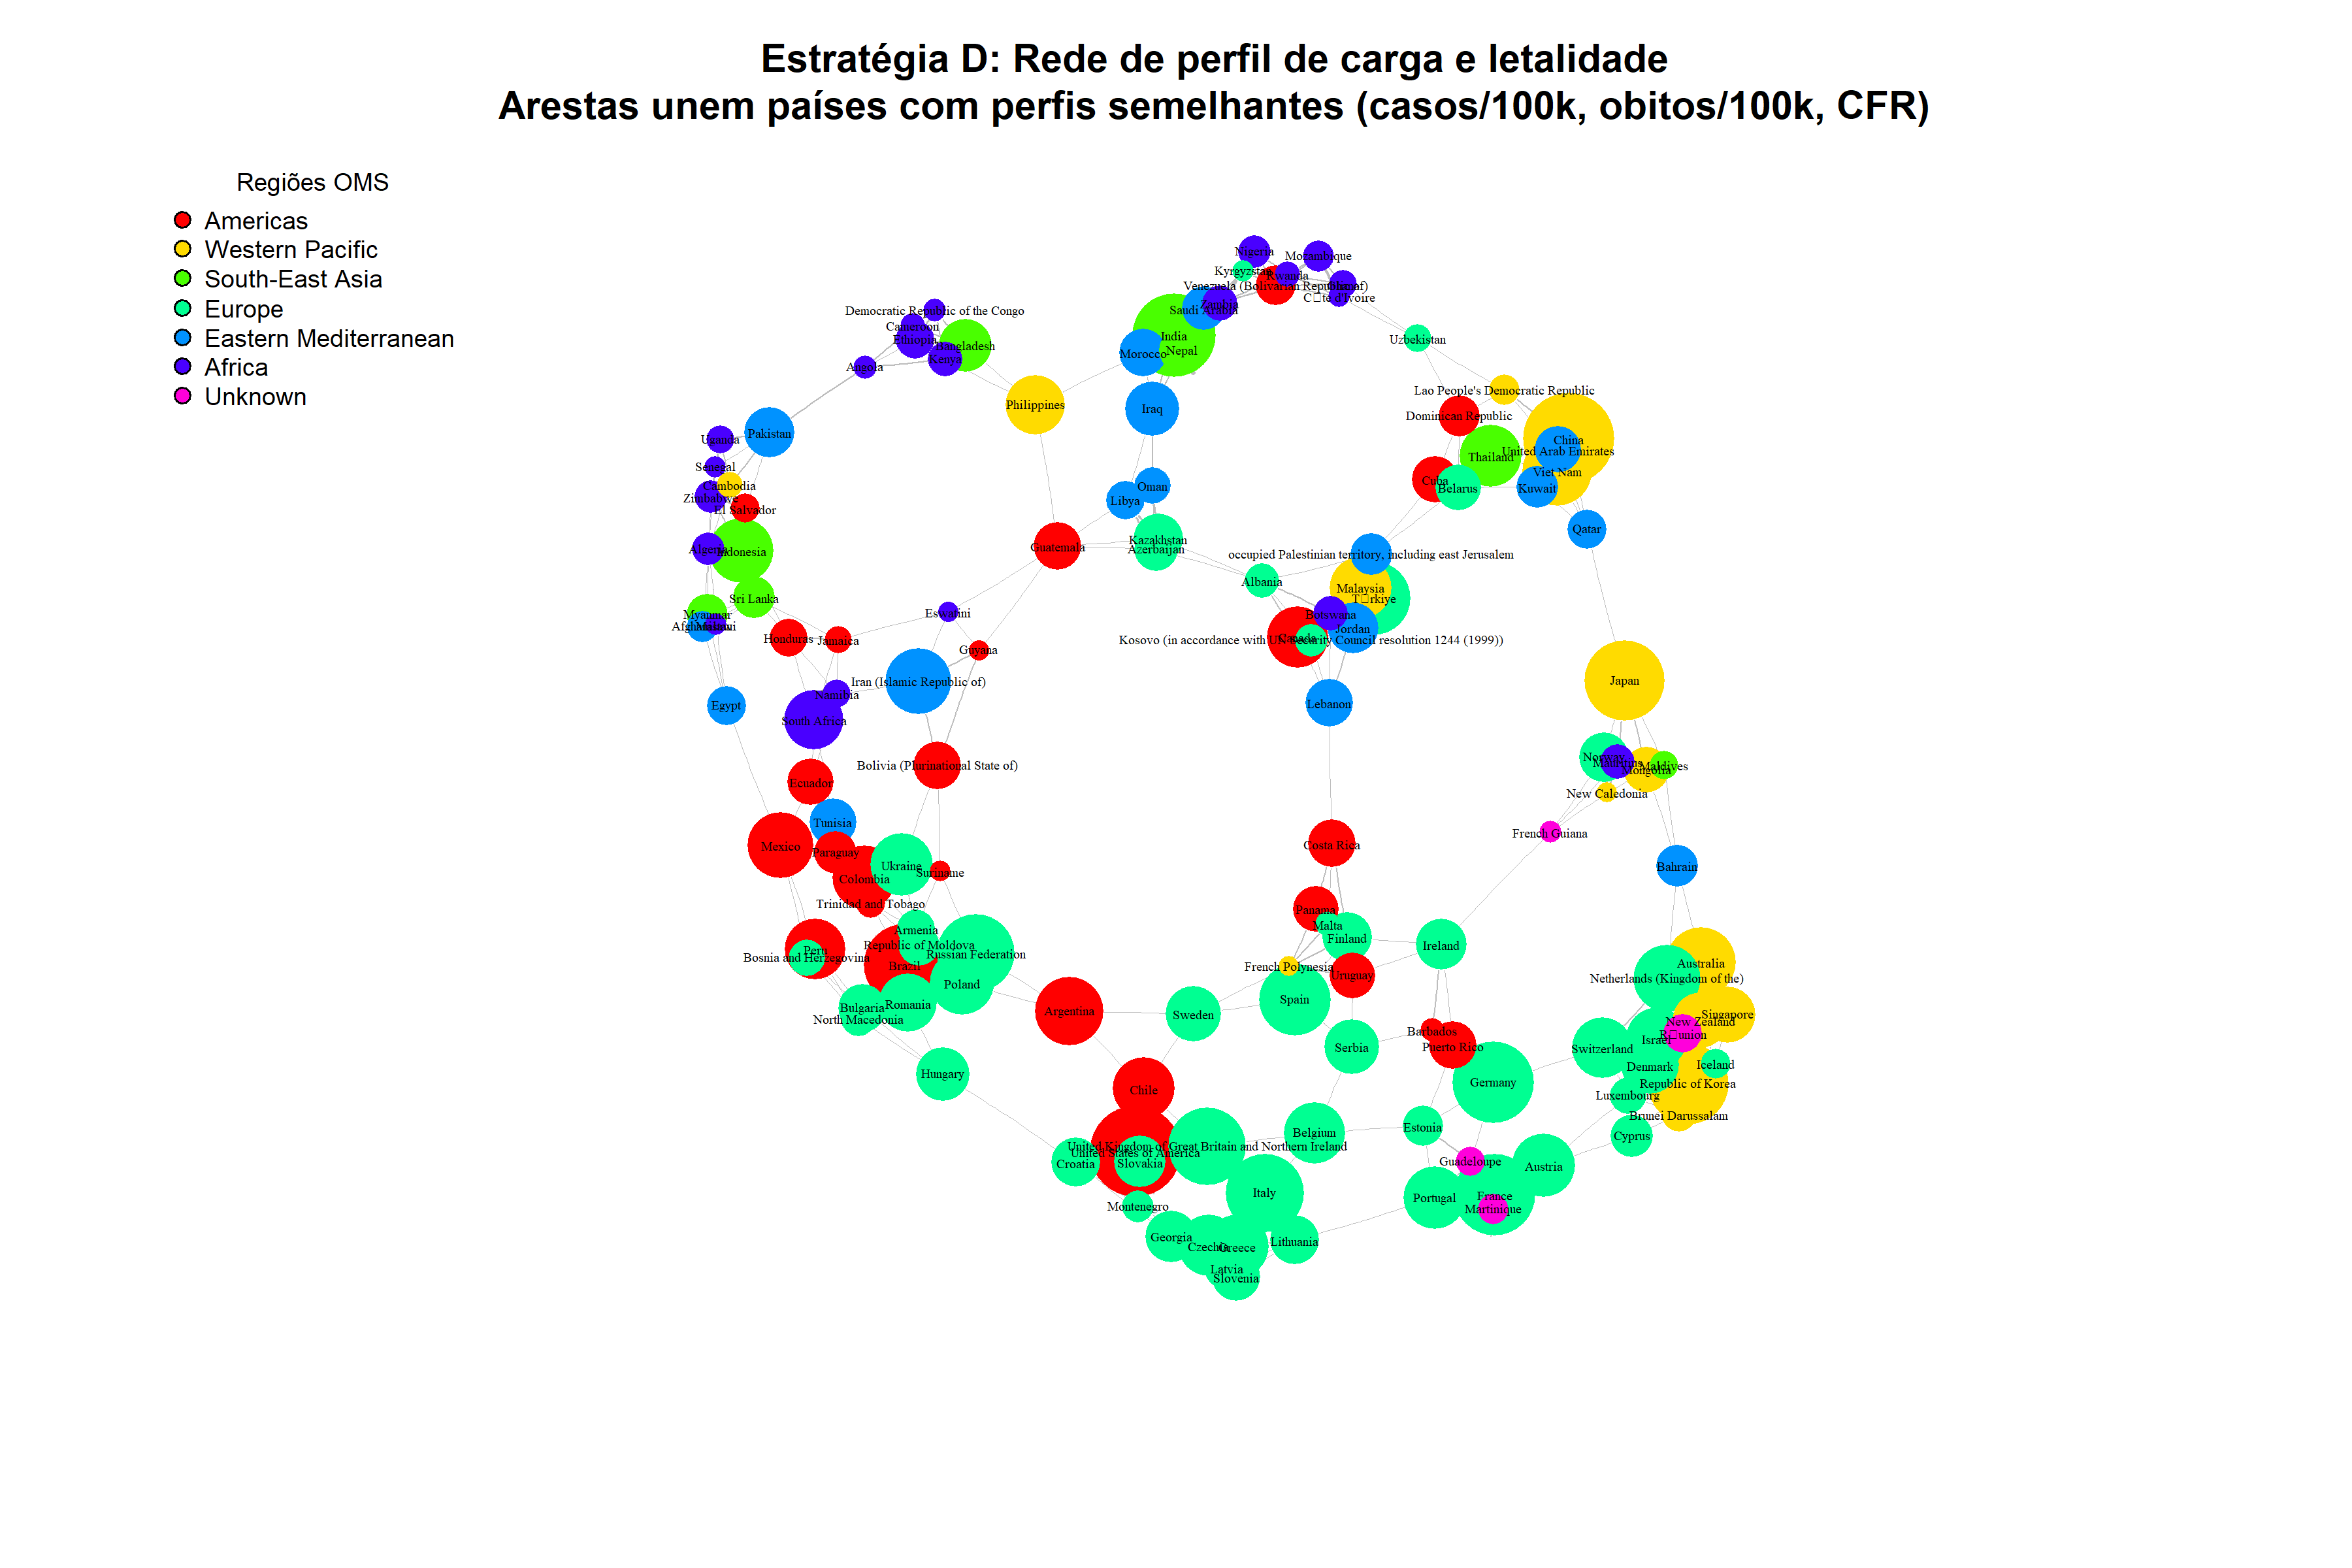
\includegraphics[width=0.98\textwidth]{rede_perfil_letalidade_carga.png}
\caption{Rede pais-pais por perfil combinado de casos por 100 mil, obitos por 100 mil e CFR.}
\end{figure}

\textbf{Interpretacao (linguagem simples):}
\begin{itemize}
  \item Essa rede mistura volume de casos, obitos e tambem o CFR (letalidade).
  \item Com isso, a analise nao fica presa so em "quem teve mais casos".
  \item Fica mais facil separar paises com carga alta daqueles com perfil mais severo.
\end{itemize}

\subsection{Estrategia E - Rede bipartida Regiao-Indicador}
\begin{figure}[H]
\centering
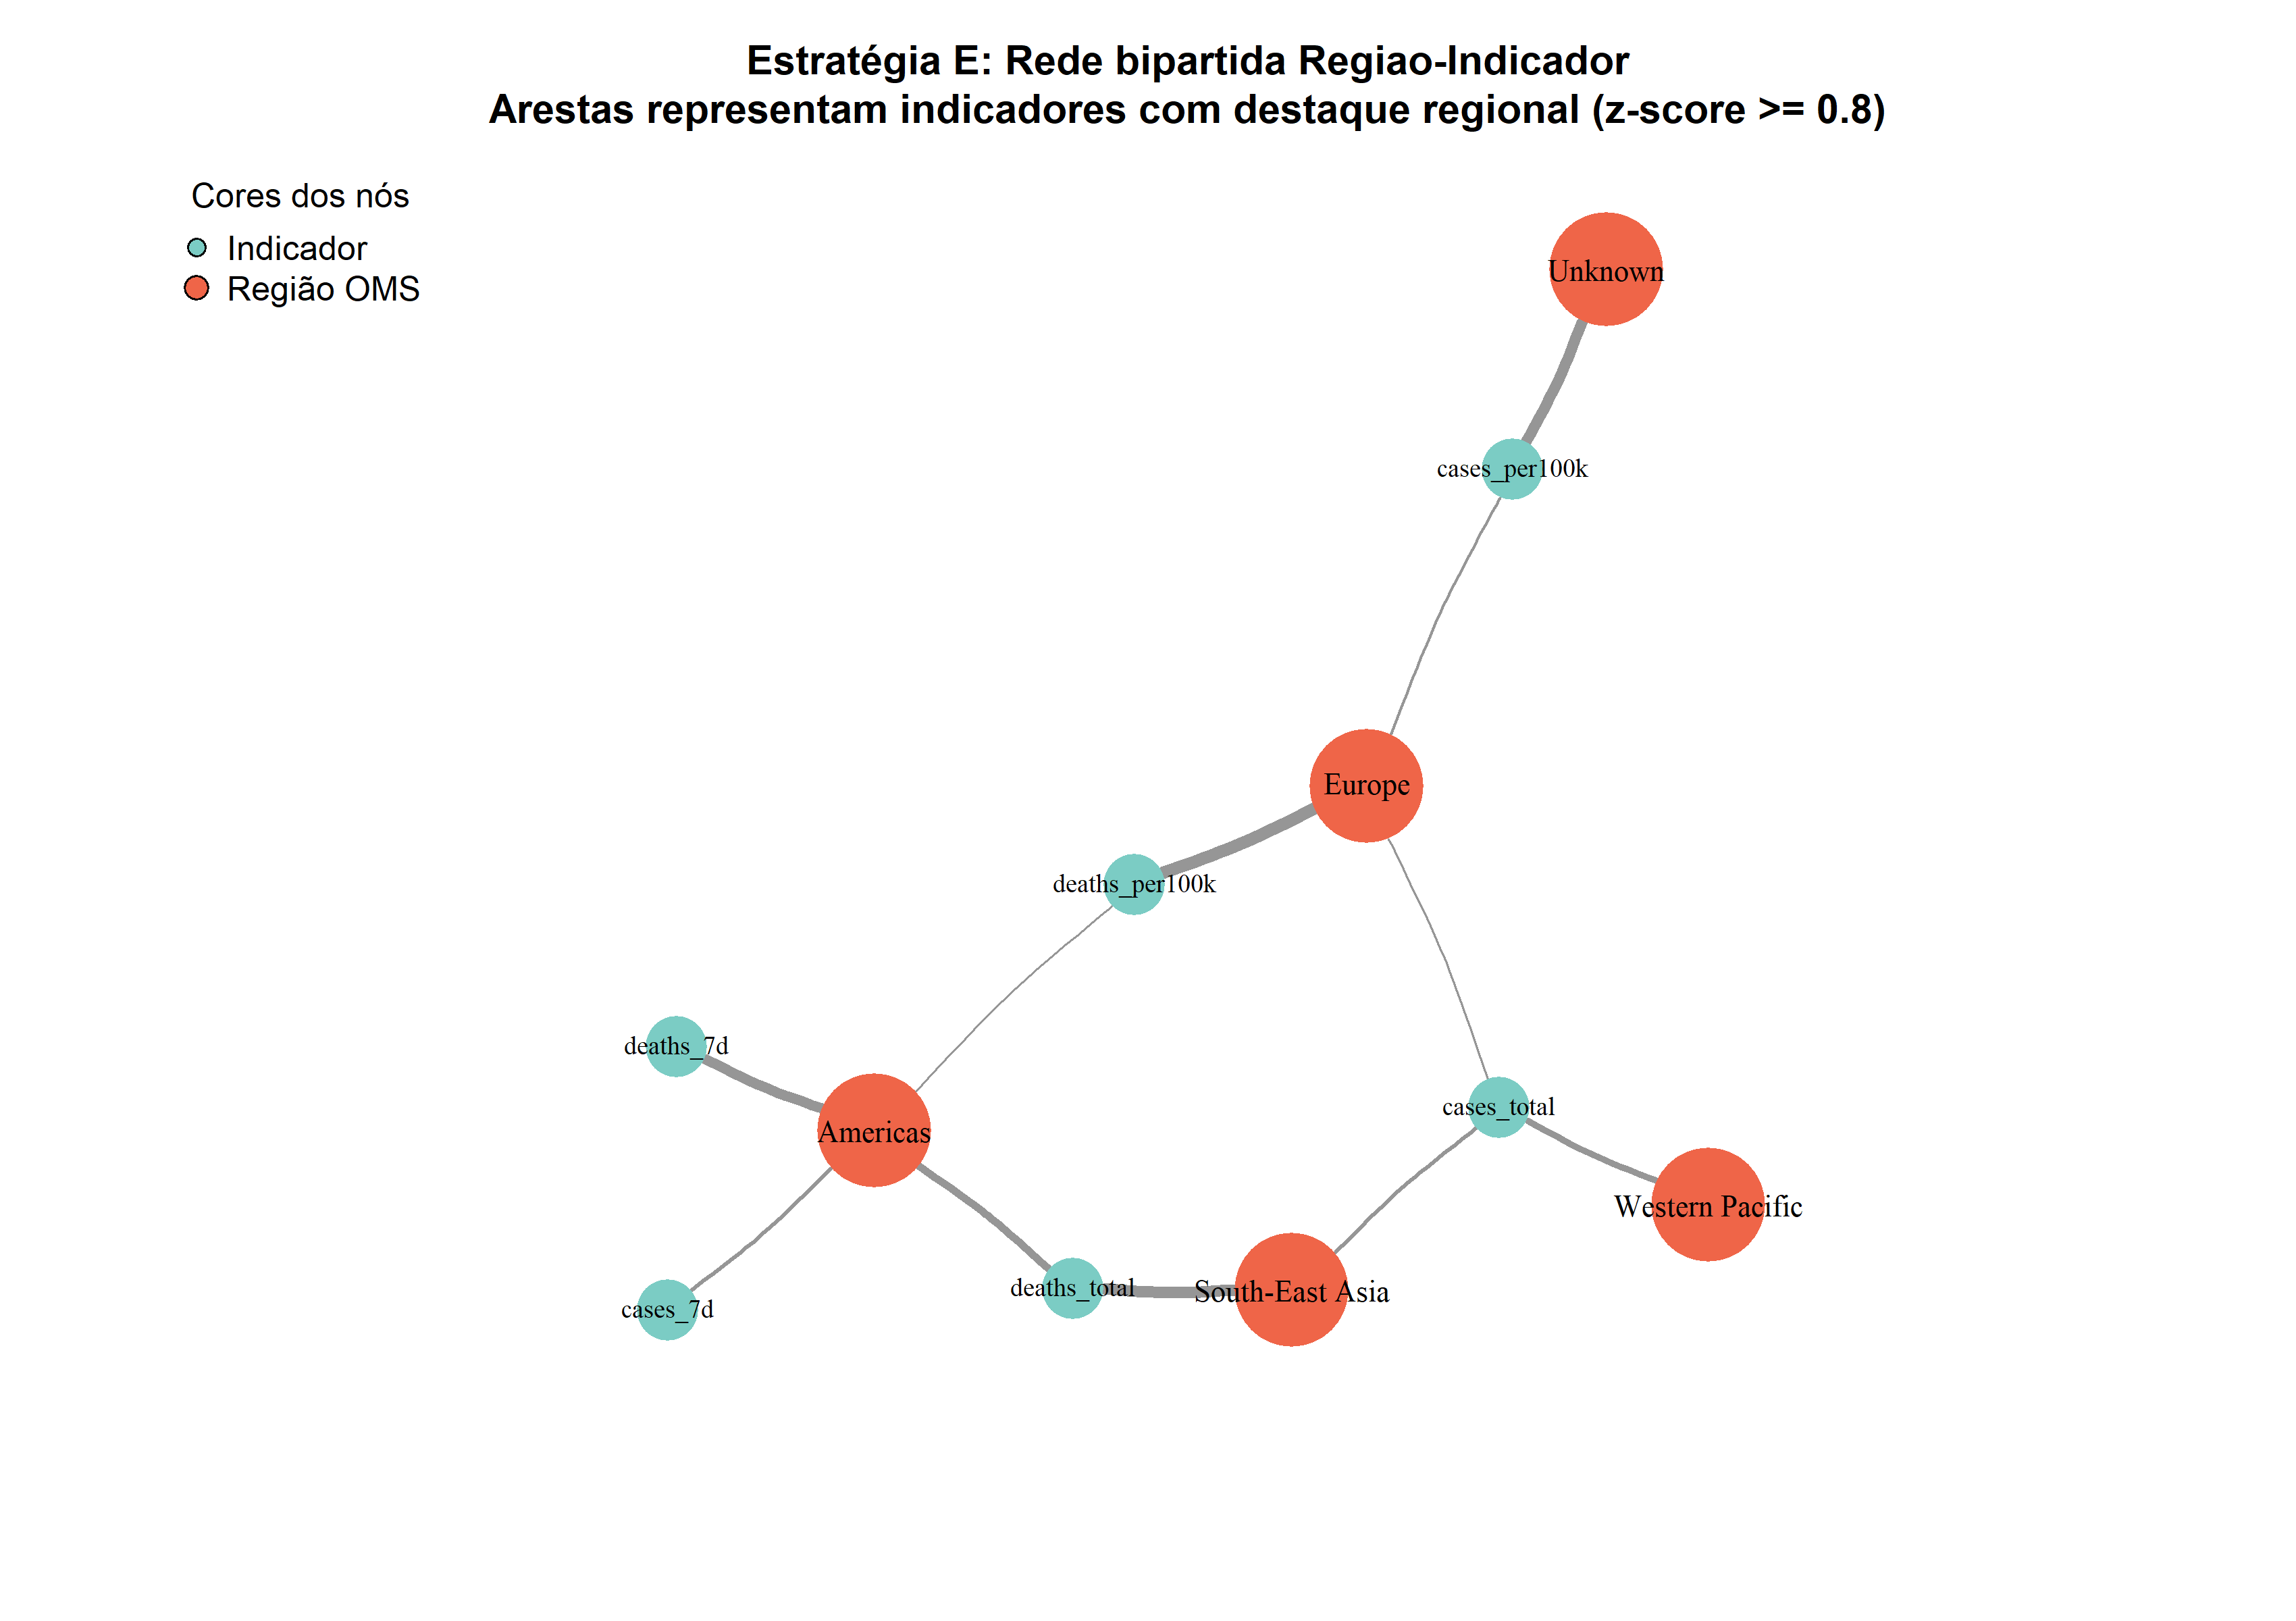
\includegraphics[width=0.98\textwidth]{rede_bipartida_regiao_indicador.png}
\caption{Rede bipartida entre regioes e indicadores com maior destaque relativo (z-score).}
\end{figure}

\textbf{Interpretacao (linguagem simples):}
\begin{itemize}
  \item Esta rede mostra quais indicadores "se destacam" em cada regiao.
  \item Funciona como um resumo rapido do perfil de cada regiao.
  \item E boa para comparar prioridades: onde chama mais atencao em casos, obitos ou indicadores recentes.
\end{itemize}

\section{Sintese dos padroes observados}
\begin{itemize}
  \item As regioes nao seguem um unico padrao; existe bastante diferenca entre elas.
  \item Na rede de comunidades (Estrategia C), vimos paises distantes com comportamento epidemiologico parecido.
  \item A Estrategia D ajudou a separar melhor "quantidade" de "severidade" por causa do CFR.
  \item A Estrategia E funcionou como um painel resumido do que mais se destaca em cada regiao.
\end{itemize}

\section{Conclusao}
No geral, as redes deixaram a analise mais visual e mais facil de explicar. Em vez de trabalhar so com tabela, foi possivel enxergar conexoes, grupos e diferencas importantes entre paises e regioes. As cinco estrategias se complementam e juntas entregam uma leitura bem completa dos dados da OMS.

\end{document}
